%
% CryptoWars (TM)
%

\section{CryptoWars\texttrademark -- Quantum cryptography}\index{Quantum key distribution}\index{Quantum cryptography}\index{CryptoWars}\label{sec:cryptowars}

Undoubtedly, quantum technologies will be most impactful (and disruptive!) in the area of information security, something of fundamental importance to us all on a daily basis, vital to the world economy. Quantum technologies will be important both in terms of breaking and maintaining security, with the former mandating interest in the latter.

In Sec.~\ref{sec:homo_blind} we discussed encrypted outsourced quantum computation as an important concept in future cloud quantum computing. In this section we will step back from full-fledged distributed quantum computation, instead focussing on more elementary protocols for simple secure communication.

Today, the ability to communicate secretly with others is completely taken for granted in all but a few nations and resides in every smartphone and desktop PC. Furthermore, the encryption technologies available to the average consumer are extremely strong, the same as those used by large organisations, including world governments.

%
% What is Security?
%

\subsection{What is security?}\index{Computational security}\index{Information-theoretic security}\label{sec:comp_vs_inf_th_sec}

Before describing any specific cryptographic protocols, let us define what is meant by `security' in a cryptographic context. We differentiate between \textit{information theoretic security}\index{Information-theoretic security}, as opposed to \textit{computational security}\index{Computational security}.

In the former, the laws of quantum information bound the amount of information that can be extracted from a system, irrespective of measurement or computational operations. Thus, such security can be regarded as attack-independent.

In the latter, security is based on the assumption that an adversary's computational resources are insufficient to perform cryptanalysis or brute-force cracking. Clearly the former makes a far stronger statement about the security of a protocol than the latter.

Classical public- and private-key encryption protocols are typically based upon the assumption of computational security (e.g the computational complexity of performing integer factorisation in the case of RSA public-key encryption, or solving a complex satisfiability problem in the case of private-key encryption), whereas quantum encryption protocols are typically information theoretically secure (e.g the one-time pad using QKD).

%
% Classical Cryptography
%

\subsection{Classical cryptography}\index{Classical cryptography}

We begin with an introduction into \textit{classical} cryptography, so as to understand its limitations, which logically leads us into how quantum mechanics can assist in overcoming these limitations. We only scratch the surface of these extremely well-researched field, reviewing some of the most important and widely used protocols. For a deeper understanding of classical cryptography we refer the interested reader to \cite{bib:Schneier96}.

%
% Private-Key Cryptography
%

\subsubsection{Private-key cryptography}\index{Private-key cryptography}

Private- (or symmetric-) key cryptography is perhaps the most basic (and useful) cryptographic primitive, enabling encryption of a channel between two parties who share a secret key\index{Secret key} -- a random bit-string of length determined by the encryption algorithm. The same secret key is employed for both encryption and decryption operations, making it of utmost importance that it be retained secret.

Private key cryptography has a long history, in fact going back to ancient times, enabling the secret sharing of diplomatic messages between emperors and empires, e.g the so-called \textit{Caesar cipher}\index{Caesar cipher}, a simple substitution cipher\index{Substitution cipher} based on shifting the letters of the alphabet. However it was a niche technology that very few utilised, since it had to be implemented by hand without computers.

Today there are countless freely available private-key cryptographic protocols available online, and some have been standardised by standards institutes. Currently, the Advanced Encryption Standard (AES) is a standard endorsed by the US government, replacing the earlier standardised Data Encryption Standard (DES)\index{Data encryption standard} whose mere 56-bit key-length is today considered insecure. AES is a block cipher\index{Block cipher}, meaning that it divides data into small blocks of 128 bits, each of which are encrypted independently, and operates with key lengths of up to 256 bits, making it very robust against (even quantum) brute-force attacks (Sec.~\ref{sec:attacks_on_class}). The length of the plaintext and ciphertext is the same, meaning there is no bandwidth overhead when communicating encrypted data across a network.

%
% One-Time Pad Cipher
%

\subsubsection{One-time pad cipher}\index{One-time pad cipher}

There is one and only one \textit{provably} secure (in the sense of information-theoretic security\index{Information-theoretic security} as opposed to computational security\index{Computational security}) encryption protocol -- the \textit{one-time pad}\index{One-time pad cipher}. This protocol requires Alice and Bob to share a random secret key as long as the message (plaintext\index{Plaintext}) being communicated between them. The two bit-strings undergo bit-wise XOR operations to form the ciphertext\index{Ciphertext}. Mathematically,\index{One-time pad cipher}
\begin{align}
c = s \oplus k,
\end{align}
where $\oplus$ is the bitwise XOR operation (equivalently addition modulo 2), and $c$, $s$ and $k$ are the ciphertext, plaintext and key bit-strings respectively, all of which are of the same length,
\begin{align}
	|c|=|s|=|k|.
\end{align}

The security of this protocol is easy to see intuitively -- with an appropriate choice of key, \textit{any} plaintext of the same length could be inferred from the ciphertext. This means that there is no possibility of performing any kind of frequency analysis\index{Frequency analysis}, as the ciphertext string has maximum entropy\index{Entropy} (inherited from the maximum entropy of the key, and assuming a strong cryptographic random bit generator) and thus no correlations. Since every possible valid plaintext can be recovered using an appropriate key, a cracking algorithm is unable to find a unique plaintext matching the ciphertext, since all are equally valid decryptions.

Importantly, the secrecy of the one-time pad\index{One-time pad cipher} strictly requires that a key never be reused. A fresh key must be generated for each message sent, otherwise trivial frequency analysis\index{Frequency analysis} techniques can be employed to compromise security. If the same key $k$ is used to encode two messages $s_1$ and $s_2$, yielding ciphertexts,
\begin{align}
c_1&=s_1\oplus k,\nonumber\\
c_2&=s_2\oplus k,
\end{align}
then we trivially obtain,
\begin{align}
c_1 \oplus c_2 &= (s_1 \oplus k) \oplus (s_2 \oplus k) \nonumber \\
&= (s_1 \oplus s_2) \oplus (k \oplus k) \nonumber \\
&= s_1 \oplus s_2,
\end{align}
which is independent of the key. Now a frequency analysis on the bitwise XOR of two plaintexts can be applied, without requiring any knowledge of the key whatsoever.

Needless to say, the requirement for keys of the same length as the plaintexts, which cannot be reused, raises the obvious criticism that now secret key-sharing is as difficult as sharing a secret message in the first place. This reduces the problem of perfect secrecy of arbitrary messages to the secrecy of shared randomness. 

Although during the Cold War Soviet diplomats would literally carry briefcases between countries full of paper with random data for use in a one-time pad, it is clearly not suitable for everyday applications!

%
% Public-Key Cryptography
%

\subsubsection{Public-key cryptography}\index{Public-key cryptography}

While private-key cryptography solves the problem of end-to-end cryptography, it has one main downfall -- how does one share a private key between two parties? After all, if we had the ability to secretly share keys between ourselves, wouldn't we just use that method to directly communicate, bypassing the unnecessary cryptographic protocol?

Public- (or asymmetric-) key cryptography addresses this issue by replacing the private key with two keys (known as a key-pair\index{Key-pair}), one used solely for \textit{encryption}, the other solely for \textit{decryption}. Importantly, these two keys are non-trivially related and cannot be efficiently computed from one another. To send a message to a friend I can send him my encryption (public) key that he is only able to use for preparing an encrypted message for me. No security is required when sharing the public key since an eavesdropper can't use it for decryption. Finally, I am able to decrypt the message using my decryption (private) key, which I kept completely to myself and never shared with anyone.

RSA \cite{bib:RSA} was the first published public-key cryptographic protocol, and forms the backbone for most encryption used on the internet today. It achieves its security based on the belief that factorising large integers into constituent primes is a computationally hard problem -- a so-called `trapdoor function'\index{Trapdoor function}. The algorithm is built upon number theory using modular arithmetic, described in detail in Alg.~\ref{alg:RSA}.

\begin{table}[!htb]
\fbox{\parbox{0.965\columnwidth}{\texttt{ 
function RSAGenerateKey():
\begin{enumerate}
\item $p$ = randomPrime()
\item $q$ = randomPrime()
\item if($p=q$) goto 1
\item $n = pq$
\item $\lambda = \text{lcm}(p-1,q-1)$
\item $e = \text{coprime}(\lambda) \,\,\text{s.t} \,\,e<\lambda$
\item $d = e^{-1}\,(\text{mod} \, \lambda)$
\item publicKey = $\{n,e\}$
\item privateKey = $\{n,d\}$
\item keyPair = \{publicKey,privateKey\}
\item return(keyPair)
\item $\Box$	
\end{enumerate}
function RSAEncrypt(plaintext, publicKey):
\begin{enumerate}
\item $\mathtt{cipertext} = \mathtt{plaintext}^e \, (\text{mod} \, n$)
\item return(ciphertext)
\item $\Box$
\end{enumerate}
function RSADecrypt(ciphertext, privateKey):
\begin{enumerate}
\item $\mathtt{plaintext} = \mathtt{ciphertext}^d \, (\text{mod} \, n)$
\item return(plaintext)
\item $\Box$
\end{enumerate}
}}}
\caption{Number-theoretic algorithms based on modular arithmetic for RSA key generation, encryption and decryption.} \label{alg:RSA}
\end{table}

A downside of RSA is that ciphertexts are in general much longer than plaintexts, unlike private-key protocols where the ciphertext is always the same length as the plaintext. For this reason it is typically not used to directly encrypt long messages, since the memory and bandwidth overheads would be undesirable. Instead, RSA is typically employed in conjunction with private-key cryptography in a key exchange protocol\index{Key exchange protocol}. Here the public-key system communicates a private \textit{session key}\index{Session key} between parties, which is subsequently employed in a private-key protocol, without incurring the memory overhead that RSA does.  

Since RSA, numerous other public-key cryptosystems have been developed, based on different choices of trapdoor function. Most notably, elliptic curve cryptography\index{Elliptic curve cryptography} has gained much attention. However, RSA remains the most widely used and well studied public-key cipher.

To mitigate the need for constant one-on-one exchange of public-keys, many key servers\index{Key servers} exist around the globe, which maintain databases of people's public-keys. These servers are in a position of trust, vouching for the identities associated with their stored public-keys.

%
% Digital Signatures
%

\subsubsection{Digital signatures} \label{sec:dig_sig} \index{Digital signatures}

Rather than cryptographically ensuring the secrecy of messages, a user may wish to prove their identity when sending a message, such that the recipient can be certain it originated from who it says it does, and accurately conveys what they said. This is achieved using \textit{digital signatures}.

Digital signatures can be easily implemented using the RSA protocol\index{RSA protocol}, but swapping the role of the public and private keys. Now the public key can only be used for decrypting a message, and the private key can only be used for encrypting it. As before, it is computationally hard to infer one from the other. The protocol for sending and verifying a digitally signed message is shown in Alg.~\ref{alg:dig_sig}.

\begin{table}[!htb]
\fbox{\parbox{0.965\columnwidth}{\texttt{ 
function DigitalSignature(message,keyPair):
\begin{enumerate}
\item Alice prepares a short \textit{digest}\index{Digest} of her message using a cryptographic hash function\index{Hash function}, such as SHA256\index{SHA256} (Sec.~\ref{sec:hashing}),\\
	\vspace{1mm} 
	$\text{digest=SHA256(message)}$
	\item Alice encrypts the digest using her private key. This forms the `digital signature',\\
	\vspace{1mm} 
	$\text{signature = RSAEncrypt(digest,privateKey)}$
	\item Alice transmits the digital signature and original message to Bob,\\
	\vspace{1mm} 
	$\text{signedMessage = \{message,signature\}}$
	\item Bob hashes the received message,\\
	\vspace{1mm} 	
	$\text{hash=SHA256(message)}$
	\item Bob uses Alice's public-key to decrypt her digital signature,\\
	\vspace{1mm} 
	$\text{decryptedHash = RSADecrypt(signature,publicKey)}$
	\item Bob compares his calculated hash with Alice's decrypted hash for consistency. If the two hashes are identical, Bob concludes the message was authentic,\\
	\vspace{1mm} 
	$\text{if(decryptedHash=hash)}$\\
	$\,\,\text{return(pass)}$\\
	$\text{else}$\\
	$\,\,\text{return(fail)}$
	\item $\Box$
\end{enumerate}
}}}
\caption{Protocol for digitally signing a message using public-key cryptography (RSA) and a cryptographic hash function (SHA256).} \label{alg:dig_sig}
\end{table}

The key point from the security perspective is that the private key cannot be efficiently inferred from the public key. So although everyone has access to Alice's public key, no one is able to counterfeit messages since they cannot create encrypted signatures without access to her private key -- signatures can be easily verified but not created.

Because this protocol is implemented using ordinary RSA\index{RSA protocol}, albeit with reversed roles for the key-pair, it shares the same security strengths and vulnerabilities as RSA public-key cryptography (Sec.~\ref{sec:attacks_on_class}).

Like RSA cryptography, key servers\index{Key servers} exist, maintaining databases of people's public-keys and their associated identities.

%
% Hashing
%

\subsubsection{Hashing} \label{sec:hashing} \index{Hash functions}

Hash functions are functions that map a long string of arbitrary length to a short, fixed-size string with quasi-random behaviour,
\begin{align}
	f_\text{hash}:\,\{0,1\}^n \to \{0,1\}^m,
\end{align}
for an $n$-bit input and $m$-bit output hash, where $n$ is variable and $m$ is fixed. They are an example of `one-way functions'\index{One-way functions} that are computationally easy to compute in the forward direction, but extremely hard to invert. That is, given a hash, it is computationally difficult to find input strings that map to that value.

Hash functions have broad applicability throughout computer science, but here we are most interested in \textit{cryptographic hash functions} for use in cryptography, which impose strong conditions on the difficulty of inversion and their quasi-random characteristics. Most notably, changing a single bit in the input string ought to flip approximately half the bits of the hash on average.

The standard cryptographic hash function with mainstream adoption is the 256-bit Secure Hashing Algorithm (SHA256\index{SHA256}), which generates 256-bit hashes. The algorithm is extremely efficient to implement digitally, and exhibits $O(n)$ runtime for input string length $n$.

Cryptographically, hash functions are useful for creating message digests\index{Message digests}, which act as a highly condensed checksum\index{Checksum} of a document that can be utilised as a digital signature (Sec.~\ref{sec:dig_sig}).

Note that because the function in general maps longer strings to shorter ones, there are necessarily \textit{collisions}\index{Hash collisions} -- multiple inputs for a given output. However, for strong cryptographic hash functions their behaviour is sufficiently random that two distinct messages will almost certainly yield completely different hashes (even if the messages are very similar), making it all but impossible for someone to make the claim that Alice said something she did not. This property is extremely important for the security of digital signatures.

%
% Attacks On Classical Cryptography
%

\subsection{Attacks on classical cryptography}\index{Cryptographic attacks}\label{sec:attacks_on_class}

%
% Classical Attacks
%

\subsubsection{Classical attacks}

Having introduced the main classes of classical cryptographic protocols, we now turn our attention to their weaknesses and vulnerabilities.

%
% Brute-Force
%

\paragraph{Brute-force}\index{Brute-force attacks}\label{sec:brute_force_attack}

The most obvious approach to cracking a cryptosystem is to systematically try out all possible keys until we find one that correctly decodes the encrypted message. This is also the most na\"ive approach, and one which is computationally intractable for real-world key lengths. Specifically, for a key length of $k$ bits (\mbox{$k=256$} for AES), there are $2^k$ possible keys to try, and on average we will wait for $2^{k-1}$ trials before choosing the right one. Clearly an average waiting time of $2^{255}$ is not plausible!

%
% Cryptanalysis
%

\paragraph{Cryptanalysis}\index{Cryptanalysis}

Far better than waiting the age of the universe for the right key to turn up, is \textit{cryptanalysis}. Here we study patterns between input and output strings from a cipher utilising a particular key. There are many variations on this, but include techniques such as \cite{bib:Schneier96}:

\begin{itemize}
	\item Known plaintext attacks (KPA)\index{Known plaintext attack}: Through alternate means of espionage, the attacker is able to possess \textit{both} a ciphertext and its associated plaintext. Knowing both the input and output to the encryption algorithm may then reveal information about the key relating them. This technique was important to Alan Turing's successful cracking of the German Enigma encryption protocol during World War II.
	\item Chosen plaintext attack (CPA)\index{Chosen plaintext attack}: The same as a KPA except that the adversary has the ability to choose what the known plaintext is.
	\item Linear cryptanalysis\index{Linear cryptanalysis}: A technique for representing ciphers as linear systems, to which KPA are applied.
	\item Differential cryptanalysis\index{Differential cryptanalysis}: We analyse how changes in input bits propagate through the cipher to modulate output bits. Typically this type of technique operates as a CPA.
\end{itemize}
 
%
% Integer Factorisation
%
 
\paragraph{Integer factorisation}\index{Integer factorisation}

In the case of RSA encryption, whose security derives from the believed computational hardness of factorising large numbers, the most efficient known classical algorithm for integer factorisation is the general number field sieve (GNFS)\index{General number field sieve}, with time-complexity,
\begin{align} \label{eq:GNFS_scaling}
	O(\text{exp}[O(1) (\log n)^{\frac{1}{3}} (\log\log n)^{\frac{2}{3}}]),
\end{align}
which scales poorly for large $n$, keeping in mind that present-day implementations of RSA accommodate key lengths of up to 4,096 bits, as for example is implemented by the Pretty Good Privacy (PGP)\index{Pretty Good Privacy} package.

%
% Quantum Attackes
%

\subsubsection{Quantum attacks}

%
% Brute-Force
%

\paragraph{Brute-force}\index{Brute-force attacks}

A brute-force attack by a quantum computer does not offer us the exponential improvement attacker Eve might hope for. However, we can gain a quadratic improvement by cleverly exploiting Grover's search algorithm (Sec.~\ref{sec:quantum_algs})\index{Grover's algorithm}.

To do this, we treat the brute-force cracking algorithm as a satisfiability problem, similar to how Grover's is employed to enhance \textbf{NP}-complete problems. Specifically, our oracle implements the code's decryption operation, taking as input a qubit string representing the key. After decoding the message with the key, the oracle runs an appropriate test on the decrypted message to determine whether it is a legitimate decoded message. For example, it could run an English language test -- a message decoded incorrectly with the wrong key will appear very random and almost certainly won't pass such a test. The oracle tags an element passing this test, which the Grover algorithm searches for, yielding the associated key.

Note that when performing a brute-force attack against a private encryption key\index{Private-key encryption}, a quadratic speedup effectively halves the key length in terms of algorithmic runtime, since \mbox{$O(\sqrt{2^k}) = O(2^{k/2})$}. Thus, in the quantum era private key lengths will need to be doubled to maintain the same security against brute-force attacks.

This same technique of treating encryption as an oracle within a quantum search algorithm can be utilised to invert hash functions\index{Hash functions}. However, in this case there will necessarily be multiple solutions.

%
% Cryptanalysis
%

\paragraph{Cryptanalysis}\index{Cryptanalysis}

In the case of private-key cryptosystems such as AES, no quantum-enhanced cryptanalytic techniques have been described, which offer an exponential enhancement. Thus, modulo doubling key-lengths to counter a Grover attack, these cryptosystems are not regarded as being compromised by quantum computing.

%
% Integer Factorisation
%

\paragraph{Integer factorisation}\index{Integer factorisation}

In the case of RSA public-key cryptography the attack is more direct -- with access to a scalable quantum computer, Shor's algorithm\index{Shor's algorithm} can be employed to efficiently factorise large integers, allowing private keys to be retrieved from public keys. Unlike the brute-force attacks, which yielded only a quadratic enhancement, Shor's algorithm is exponentially faster than the classical GNFS, requiring runtime of only,
\begin{align}
	O([\log n]^2[\log\log n][\log\log\log n]).
\end{align}
Compare this with Eq.~(\ref{eq:GNFS_scaling}).

%
% Bitcoin & The Blockchain
%

\subsection{Bitcoin \& the Blockchain}\index{Blockchain}\index{Bitcoin}

One of the most exciting new cryptographic applications that has emerged in recent years is the Blockchain, a secure distributed ledger\index{Distributed ledger} for recording the execution of contracts and transactions. This has enabled cryptocurrencies\index{Cryptocurrencies}, most notably Bitcoin, to emerge as a secure digital alternative to conventional fiat currencies.

More recent developments, such as the Ethereum project\index{Ethereum}, develop the distributed ledger further to allow executable code to be committed to the Blockchain, opening the prospects for self-enforcement and -execution of completely arbitrary contracts, a potential game-changer for the operation of financial and derivative markets.

In the Blockchain protocol, the validity of contracts and transactions is recognised collectively by participants using an encrypted digital ledger. The ledger records the complete history of all Blockchain transactions, which are digitally signed (Sec.~\ref{sec:hashing}) by network participants using elliptic curve public-key cryptography\index{Digital signatures}\index{Elliptic curve cryptography}. A democratic process ensures that, provided a single user doesn't monopolise the network, recorded transactions are legitimate, recognised collectively. This is secured by network participants digitally signing off on transactions as they take place.

The Bitcoin protocol builds on top of the Blockchain to create a secure digital cryptocurrency. This requires the introduction of another sub-protocol, \textit{mining}\index{Bitcoin mining}, where units of currency (`coins'\index{Coins}) are created. The protocol cryptographically ensures that there is an upper-bound on the number of coins that can exist, thereby preventing forgery and an inflationary blowout in the money supply.

The mining process is based upon the computational hardness of inverting SHA256 hashing\index{Hash functions}\index{SHA256}. A legitimate Bitcoin is defined by a string with a hash satisfying a thoughtfully chosen constraint, specifically one which hashes to a value within some range,
\begin{align}
	y_\text{lower}\leq \text{SHA256}(\text{SHA256}(x_\text{coin})) \leq y_\text{upper}.
\end{align}
This is slightly weaker than inverting hash functions, but is nonetheless a task that can only be approached via brute-force hashing in the forward direction. This associates computational complexity with the mining process, and hence computational integrity of the money supply, whilst upper bounding the number of unique coins that can exist.

The two key algorithms for Bitcoin and the Blockchain are therefore hashing and public-key digital signatures. Both of these are subject to enhanced quantum attacks.

Hashing does not have any known quantum algorithm with exponential improvement, however using a Grover search\index{Grover's algorithm} one can achieve a quadratic speedup, using the same idea as for enhancing \textbf{NP}-complete problems by treating the hash function as a search oracle\index{Oracle}. This however does not pose a fundamental security concern as it will speed up the Bitcoin mining process, but does not circumvent the upper-bound on the number of coins that may be in existence. Already classical mining has pushed the Bitcoin money supply close to its asymptotic maximum and there is limited room for additional mining.

Elliptic curve public-key cryptography, like RSA, has a known efficient quantum attack via Shor's algorithm\index{Shor's algorithm}. In the context of implementing digital signatures this implies that an adversary could fraudulently sign off on illegitimate transactions, thereby committing falsified contracts to the Blockchain.

A detailed investigation into the vulnerability of the Blockchain to quantum attacks was performed by \cite{bib:TomamichelBlockchain}. However, it is near impossible to predict the future rate of growth in quantum computer technology and hence over what kind of timescale the Blockchain will be compromised. But it is certain that a full compromise is inevitable at some point in the future.

To address this security threat, quantum-resistant hashing and public-key cryptographic protocols will need to be developed. In the former case this can easily be achieved by increasing hash lengths so as to offset the quadratic enhancement offered by Grover's algorithm\index{Grover's algorithm}. In the latter case this will require post-quantum public-key cryptosystems (to be discussed in the next section).

Evidently, the lifespan of exisiting Blockchain technologies is limited and in the quantum future post-quantum Blockchain algorithms will be required to ensure the survival of cryptocurrencies.

%
% The End Of Classical Cryptography?
%

\subsection{The end of classical cryptography?} \label{sec:end_of_class_crypto}

The vulnerability of RSA to attacks by quantum computers raises the question whether this spells the end of classical cryptography and compromises the security of much of the present-day internet.

Thankfully, there are two saving graces. First of all, much research is being carried out into \textit{post-quantum classical cryptography}\index{Post-quantum classical cryptography}. That is, public-key cryptosystems based upon trapdoor functions\index{Trapdoor function} that reside outside of \textbf{BQP} and are therefore not efficiently attacked by quantum computers. One such line of research is to construct cryptosystems based upon \textbf{NP}-complete problems, such as the McEliece protocol\index{McEliece protocol}. Recall from Fig.~\ref{fig:complexity_classes} that \textbf{NP}-complete is strongly believed to reside completely outside of \textbf{BQP}. However, while many computer scientists might be comfortable with such a level of security, it is nonetheless based on the unproven conjecture that \textbf{NP}-complete and \textbf{BQP} do not intersect, i.e \mbox{$\mathbf{NP}\nsubseteq\mathbf{BQP}$}. What would be much more satisfying would be protocols demonstrating information-theoretic security\index{Information-theoretic security} rather than computational security\index{Computational security}. Here quantum mechanics can help us -- \textit{quantum cryptography}.

%
% Quantum Cryptography
%

\subsection{Quantum cryptography}\index{Quantum cryptography}

%
% Quantum Key Distribution (QKD)
%

\subsubsection{Quantum key distribution (QKD)} \label{sec:QKD} \index{Quantum key distribution (QKD)}

%Aside from quantum computing, a central use for quantum technologies is in cryptography \cite{bib:Gisin02}. The demand for secure cryptography is now extremely important in the context of electronic commerce and general security of information transmission in the internet age. Electronic currencies such as Bitcoin\index{Bitcoin} depend on cryptographic protocols in order to secure the value of assets, assign ownership certificates\index{Owner certificates}, and secure the currency against fraud. However such protocols are based upon the computational complexity of certain mathematical problems (\textit{computational security}\index{Computational security}), and are not fundamentally secure in the presence of limitless computational resources, or quantum computers. Therefore, using quantum mechanical protocols based on physical principles (\textit{information-theoretic security}\index{Information-theoretic security}) rather than computational limitations, are favourable in the sense of future-proofing security.

\comment{Add more advanced protocols? CV? Decoy states, untrusted devices, device independent QKD, etc. etc.}

Quantum key distribution (QKD) protocols facilitate shared, secret randomness, where any intercept-resend\index{Intercept-resend attack} (or man-in-the-middle attack) attack may be detected and rejected, guaranteed by the laws of quantum physics (specifically the Heisenberg uncertainty principle\index{Heisenberg uncertainty principle} and no-cloning theorem\index{No-cloning theorem}). This shared, secret randomness may subsequently be employed in a one-time pad cipher\index{One-time pad cipher}, presenting us with true information-theoretic security\index{Information-theoretic security}.

The central notion to QKD protocols, in their numerous manifestations, is that measurement of quantum states invokes a wavefunction collapse. When measuring a state in a basis for which that state is not an eigenstate, this necessarily changes the state. QKD relies on this simple result from quantum mechanics to reveal any eavesdropper performing an intercept-resend attack\index{Intercept-resend attack} via the changes to transmitted quantum states that this would induce.

QKD is a relatively mature technology with already several commercial systems being available off-the-shelf\footnote{\cite{??? example companies}} and initial space-based implementations have been successfully demonstrated \cite{Pan}.

It is easy to see the utility of quantum networks in enabling commodity deployment of QKD -- users desire to communicate photons across long-range ad hoc networks, with low loss and dephasing. A global quantum internet would allow quantum cryptography to truly supersede classical cryptography, bypassing the vulnerabilities faced by classical cryptography in the era of quantum computing.

In Sec.~\ref{sec:state_of_the_art} we summarise the state-of-the-art in the physical implementation of QKD.

%
% BB84 Protocol
%

\paragraph{BB84 protocol}\index{BB84 protocol}

The first described QKD scheme was the \textit{BB84} \cite{bib:BennetBrassard84}\index{BB84 protocol} protocol, which exploits the fact that states encoded in the $\hat{Z}$-basis but measured in the $\hat{X}$-basis (and vice versa) collapse randomly, yielding completely random measurement outcomes, whereas states measured in the same basis in which they were encoded always correctly communicate a single bit of information.

Implemented photonically, BB84 requires only the transmission of a sequence of single photons, polarisation-encoded\index{Polarisation encoding} with random data.

The BB84 protocol is described in detail in Alg.~\ref{alg:bb84} in the context of polarisation-encoded photons, which is the most natural (but not only) setting for this protocol. An example evolution of the protocol is illustrated in Fig.~\ref{fig:BB84_example}

\begin{table}[!htb]
\fbox{\parbox{0.965\columnwidth}{\texttt{ 
function BB84():
\begin{enumerate}
\item Alice chooses a random bit, $0$ or $1$.
\item Alice randomly chooses a basis, $\hat{X}$ or $\hat{Z}$.
\item Depending on the choice of basis, she encodes her bit into the polarisation of a single photon as:
\begin{align}
\ket{0}_Z &\equiv \ket{H}, \nonumber \\
\ket{1}_Z &\equiv \ket{V},
\end{align}
or,
\begin{align}
\ket{0}_X &\equiv \frac{1}{\sqrt{2}}(\ket{H}+\ket{V}), \nonumber \\
\ket{1}_X &\equiv \frac{1}{\sqrt{2}}(\ket{H}-\ket{V}).
\end{align}
\item Encoding into the randomly chosen basis, she transmits the randomly chosen bit to Bob.
\item She does not announce the choice of bit or basis.
\item Bob measures the bit in a randomly chosen basis, $\hat{X}$ or $\hat{Z}$.
\item The above is repeated many times.
\item Upon receipt of all qubits, Alice (publicly) announces the basis used for encoding each bit sent.
\item Qubits where Bob measured in the opposite basis to which Alice encoded are discarded, as they will be decorrelated from Alice.
\item The remaining measurement outcomes are guaranteed to yield identical bits between Alice and Bob.
\item Remaining is roughly half as many bits as were sent, which are random, but guaranteed to be identical between Alice and Bob.
\item Alice and Bob sacrifice some of their bits by publicly communicating them to check for consistency. This rules out intercept-resend attacks.
\item Privacy amplification may be used to distill the partially compromised key into a shorter but more secret one.
\end{enumerate}}}}
\caption{BB84\index{BB84 protocol} QKD protocol using polarisation-encoded\index{Polarisation encoding} photons. Upon completion of the protocol, Alice and Bob share a random bit-string for use in a one-time pad cipher\index{One-time pad cipher}.}\label{alg:bb84}
\end{table}

\begin{figure}[!htb]

\includegraphics[width=0.47\textwidth]{BB84_example}
\caption{Example execution of the BB84 protocol for securely sharing random bit-strings between Alice and Bob as per Alg.~\ref{alg:bb84}. At the conclusion of the protocol, some bits are discarded (X), with those remaining guaranteed to be secret between the two parties.} \label{fig:BB84_example}	
\end{figure}

To understand the secrecy of the protocol as described in Alg.~\ref{alg:bb84}, suppose an eavesdropper, Eve, were to perform an intercept-resend\index{Intercept-resend attack} attack on the channel between Alice and Bob. At that stage in the protocol Alice had not yet announced her choice of encoding bases, and Eve will not know the bases in which to measure states without randomly collapsing them onto values inconsistent with Alice's encoding. Thus, by sacrificing some of their shared bits, via openly communicating them to one another for comparison, such an attack will be detected with asymptotically high security. Now Alice and Bob have great confidence that they have a shared, secret, random bit-string, which may subsequently be employed in a one-time pad\index{One-time pad cipher} with perfect secrecy.

The BB84 protocol has no measurement timing, mode-matching or interferometric stability requirements, making it a very robust protocol, readily achievable with present-day photonics technology. The scheme has been adapted to physical architectures beyond just polarisation-encoded photons, such as CV encodings\index{Continuous-variable QKD} \cite{???}.

%
% E91 Protocol
%

\paragraph{E91 protocol}\index{E91 protocol}

E91 is slightly different to BB84. Here Alice and Bob share an entangled Bell-pair provided by a central authority. Then both Alice \textit{and} Bob measure their qubits in random bases. As with BB84, after measuring all qubits, they compare their choices of random bases. When they coincide, they have a shared, random bit. When they don't, they discard their result. From here the remainder of the protocol is the same as for BB84. Thre protocol is summarised in Alg.~\ref{alg:e91}.

\begin{table}[!htb]
\fbox{\parbox{0.965\columnwidth}{\texttt{ 
function E91():
\begin{enumerate}
\item A central server shares a Bell-pair between Alice and Bob,
\begin{align}
\ket{\Phi^+} = \frac{1}{\sqrt{2}}(\ket{0}_A\ket{0}_B+\ket{1}_A\ket{1}_B).
\end{align}
\item Alice randomly measures her qubit in either the $\hat{X}$ or $\hat{Z}$ basis.
\item Bob randomly measures his qubit in either the $\hat{X}$ or $\hat{Z}$ basis.
\item Alice and Bob share what their measurement bases were (classically and unencrypted).
\item When Alice and Bob's bases were consistent they store the measurement outcomes as a shared random bit.
\item Alice and Bob sacrifice some of their bits by publicly communicating them to check for consistency. This rules out intercept-resend attacks.
\item Privacy amplification may be used to distill the partially compromised key into a shorter but more secret one.
\end{enumerate}}}}
\caption{E91\index{E91 protocol} QKD protocol using polarisation-encoded\index{Polarisation encoding} photonic Bell-pairs. Upon completion of the protocol, Alice and Bob share a random bit-string of ruse in a one-time pad cipher\index{One-time pad cipher}.}\label{alg:e91}
\end{table}

\comment{Explain privacy amplification}

\comment{What's the other QKD protocol? Include it}

Like BB84, E91 has no mode-matching\index{Mode-matching} or interferometric stability\index{Interferometric stability} requirements, and Alice and Bob both only require single-photon detection. Unlike BB84, however, E91 requires a central authority that is able to prepare entanglement on-demand as a resource.

An advantage of E91 over BB84 is that it does not require a direct quantum communications link between Alice and Bob. The protocol could be mediated from above by a Bell-pair-producing satellite within line-of-sight of both Alice and Bob.

%
% Continuous-Variable Protocols
%

\paragraph{Continuous-variable protocols}

\comment{To do. Zixin perhaps??}

%
% Security
%

\paragraph{Security}\index{Security of QKD}

Importantly, unlike classical cryptographic protocols, QKD makes no assumptions about the computational complexity of inverting encoding algorithms or trapdoor functions. The protocols are information-theoretically secure\index{Information-theoretic security}, and therefore no physically realisable computer, even a quantum computer, can compromise them. Thus, usual cryptanalytic techniques, like linear and differential cryptanalysis \cite{bib:Schneier96}\index{Linear cryptanalysis}\index{Differential cryptanalysis}, or the ability to factor large numbers\index{Integer factorisation}, that are employed to attack other encryption protocols, do not compromise QKD.

However, this is not to say that QKD is actually perfectly secure in real life. Recent history has demonstrated that this is certainly not the case, with many attacks against various quantum cryptographic protocols being described and successfully demonstrated. The reason for this schism between theory and experiment is that no experiment ever \textit{perfectly} mimics the theoretical proposal it is trying to implement. Laboratory components might be imprecise in an unfortunate way, opening up avenues for attack, or they might perform unwanted additional actions that leak information to Eve.

The best known attack against photonically implemented BB84 is the `photon-number splitting attack'\index{Photon-number splitting attack}. This attack targets implementations where Alice's photon source does not produce perfect single-photon states, but may have some amplitude of higher photon-number. Weak coherent states or SPDC states exhibit this property. The attack is very simple. Eve simply performs a man-in-the-middle attack\index{Man-in-the-middle attack}, but not of an intercept-resend\index{Intercept-resend attack} variety. Rather than intercepting the entire channel, she inserts a low reflectivity beamsplitter and measures only the reflected mode, the other following its desired trajectory to Bob. Now there is a chance that Eve can extract just one of the multiple photons in the signal, such that Bob still receives a photon. Eve holds the split-off signal in memory until the classical communication of encoding bases, at which point she measures all her split signals in the correct basis.

This trivial attack vector clearly demonstrates the importance of well-considered engineering decisions when physically implementing QKD. No piece of hardware is ever 100\% to specification!

\comment{Decoy states}

%
% Hybrid Quantum/Classical Cryptography
%

\subsubsection{Hybrid quantum/classical cryptography}\index{Hybrid quantum/classical cryptography}

As discussed, the RSA public-key cryptosystem is vulnerable to an efficient quantum attack, whereas private-key schemes like AES are not (believed to be). Thus, combining QKD schemes with private-key classical schemes does not compromise security in the quantum era.

Why would we combine quantum and classical encryption techniques when QKD is already provably secure, whereas the classical schemes are not?

In the near future, as QKD schemes begin their rollout in space and on Earth, random bits from the QKD implementation will be very expensive and exhibit low bandwidth. Suppose we wanted to securely videoconference across the globe. For just a single user this would require megabits per second of shared random bits, which will quickly saturate the capacity of overhead quantum satellites. Instead, let us use the QKD system to securely share just a 256-bit private session key\index{Session key} between two users. This is subsequently employed for AES256 encryption that operates entirely over the classical network, which we regard as extremely cheap. Importantly, unlike one-time pad implementations, this session key may be reused. Now we have a hybrid system which is not quantum-compromised, but which overcomes the cost and bandwidth issues associated with upcoming QKD networks.

While such a hybrid scheme is not information-theoretically secure (AES is not proven to be quantum-safe), the computational security assumptions are far stronger than for say RSA, since there are no known efficient quantum attacks against strong private-key schemes.

%
% Quantum Anonymous Broadcasting
%

\subsubsection{Quantum anonymous broadcasting} \label{sec:anon_broad} \index{Quantum anonymous broadcasting}

The previously described protocols all focussed on preserving the secrecy of messages. Alternately, it may not be the message that is sensitive, but rather the identity of the person who says it. \textit{Anonymous broadcasting}\index{Anonymous broadcasting} is a protocol for achieving this.

Consider the following scenario. A group of users share a classical broadcast channel that anyone is able to transmit to, and everybody is able to listen to unencrypted. But it is of importance that the identity of whoever broadcasts to the channel must be kept secret from all users. \cite{Wehner} described a scheme for achieving this quantum mechanically using shared GHZ states -- \textit{quantum anonymous broadcasting} (QAB).

Let there be a (trusted) server that distributes GHZ states (of arbitrary numbers of qubits) to a group of users, one qubit per user. This can be prepared as described in, for example, Sec.~\ref{sec:GHZ_states}. Now if every user measures in the \mbox{$\ket\pm=\frac{1}{\sqrt{2}}(\ket{0}+\ket{1})$} basis the joint \textit{parity} (i.e whether an even or odd number of $+$'s were measured) is guaranteed to be even. For example, all users might measure $\ket{+}\bra{+}$, or exactly 2, but never exactly 1 or 3.

On the other hand, if a $\hat{Z}$ gate were applied to any one qubit, this would flip the parity outcome. Note that a GHZ transforms according to,
\begin{align}
	\hat{Z}_i \frac{1}{\sqrt{2}}(\ket{0}^{\otimes n} + \ket{1}^{\otimes n}) \to \frac{1}{\sqrt{2}}(\ket{0}^{\otimes n} - \ket{1}^{\otimes n})\,\,\forall \, i,
\end{align}
for any qubit $i$. This invariance in the location of the $\hat{Z}$ gate is the basis for the anonymity of the protocol. If a user wishes to broadcast `0' he does nothing, whereas if he wishes to broadcast `1' he applies the $\hat{Z}$ gate to his local qubit.

Finally, all users measure their qubits in the $\pm$-basis and publicly (without encryption) broadcast their measurement outcomes. All users now see all other users' measurement outcomes and are able to calculate the collective parity of the measurements. Now if the parity is even, the speaker must have said `0', whereas if it is odd he must have said `1'. The protocol is shown in Fig.~\ref{fig:QAB} and described in detail in Alg.~\ref{alg:QAB}.

\begin{figure}[!htb]
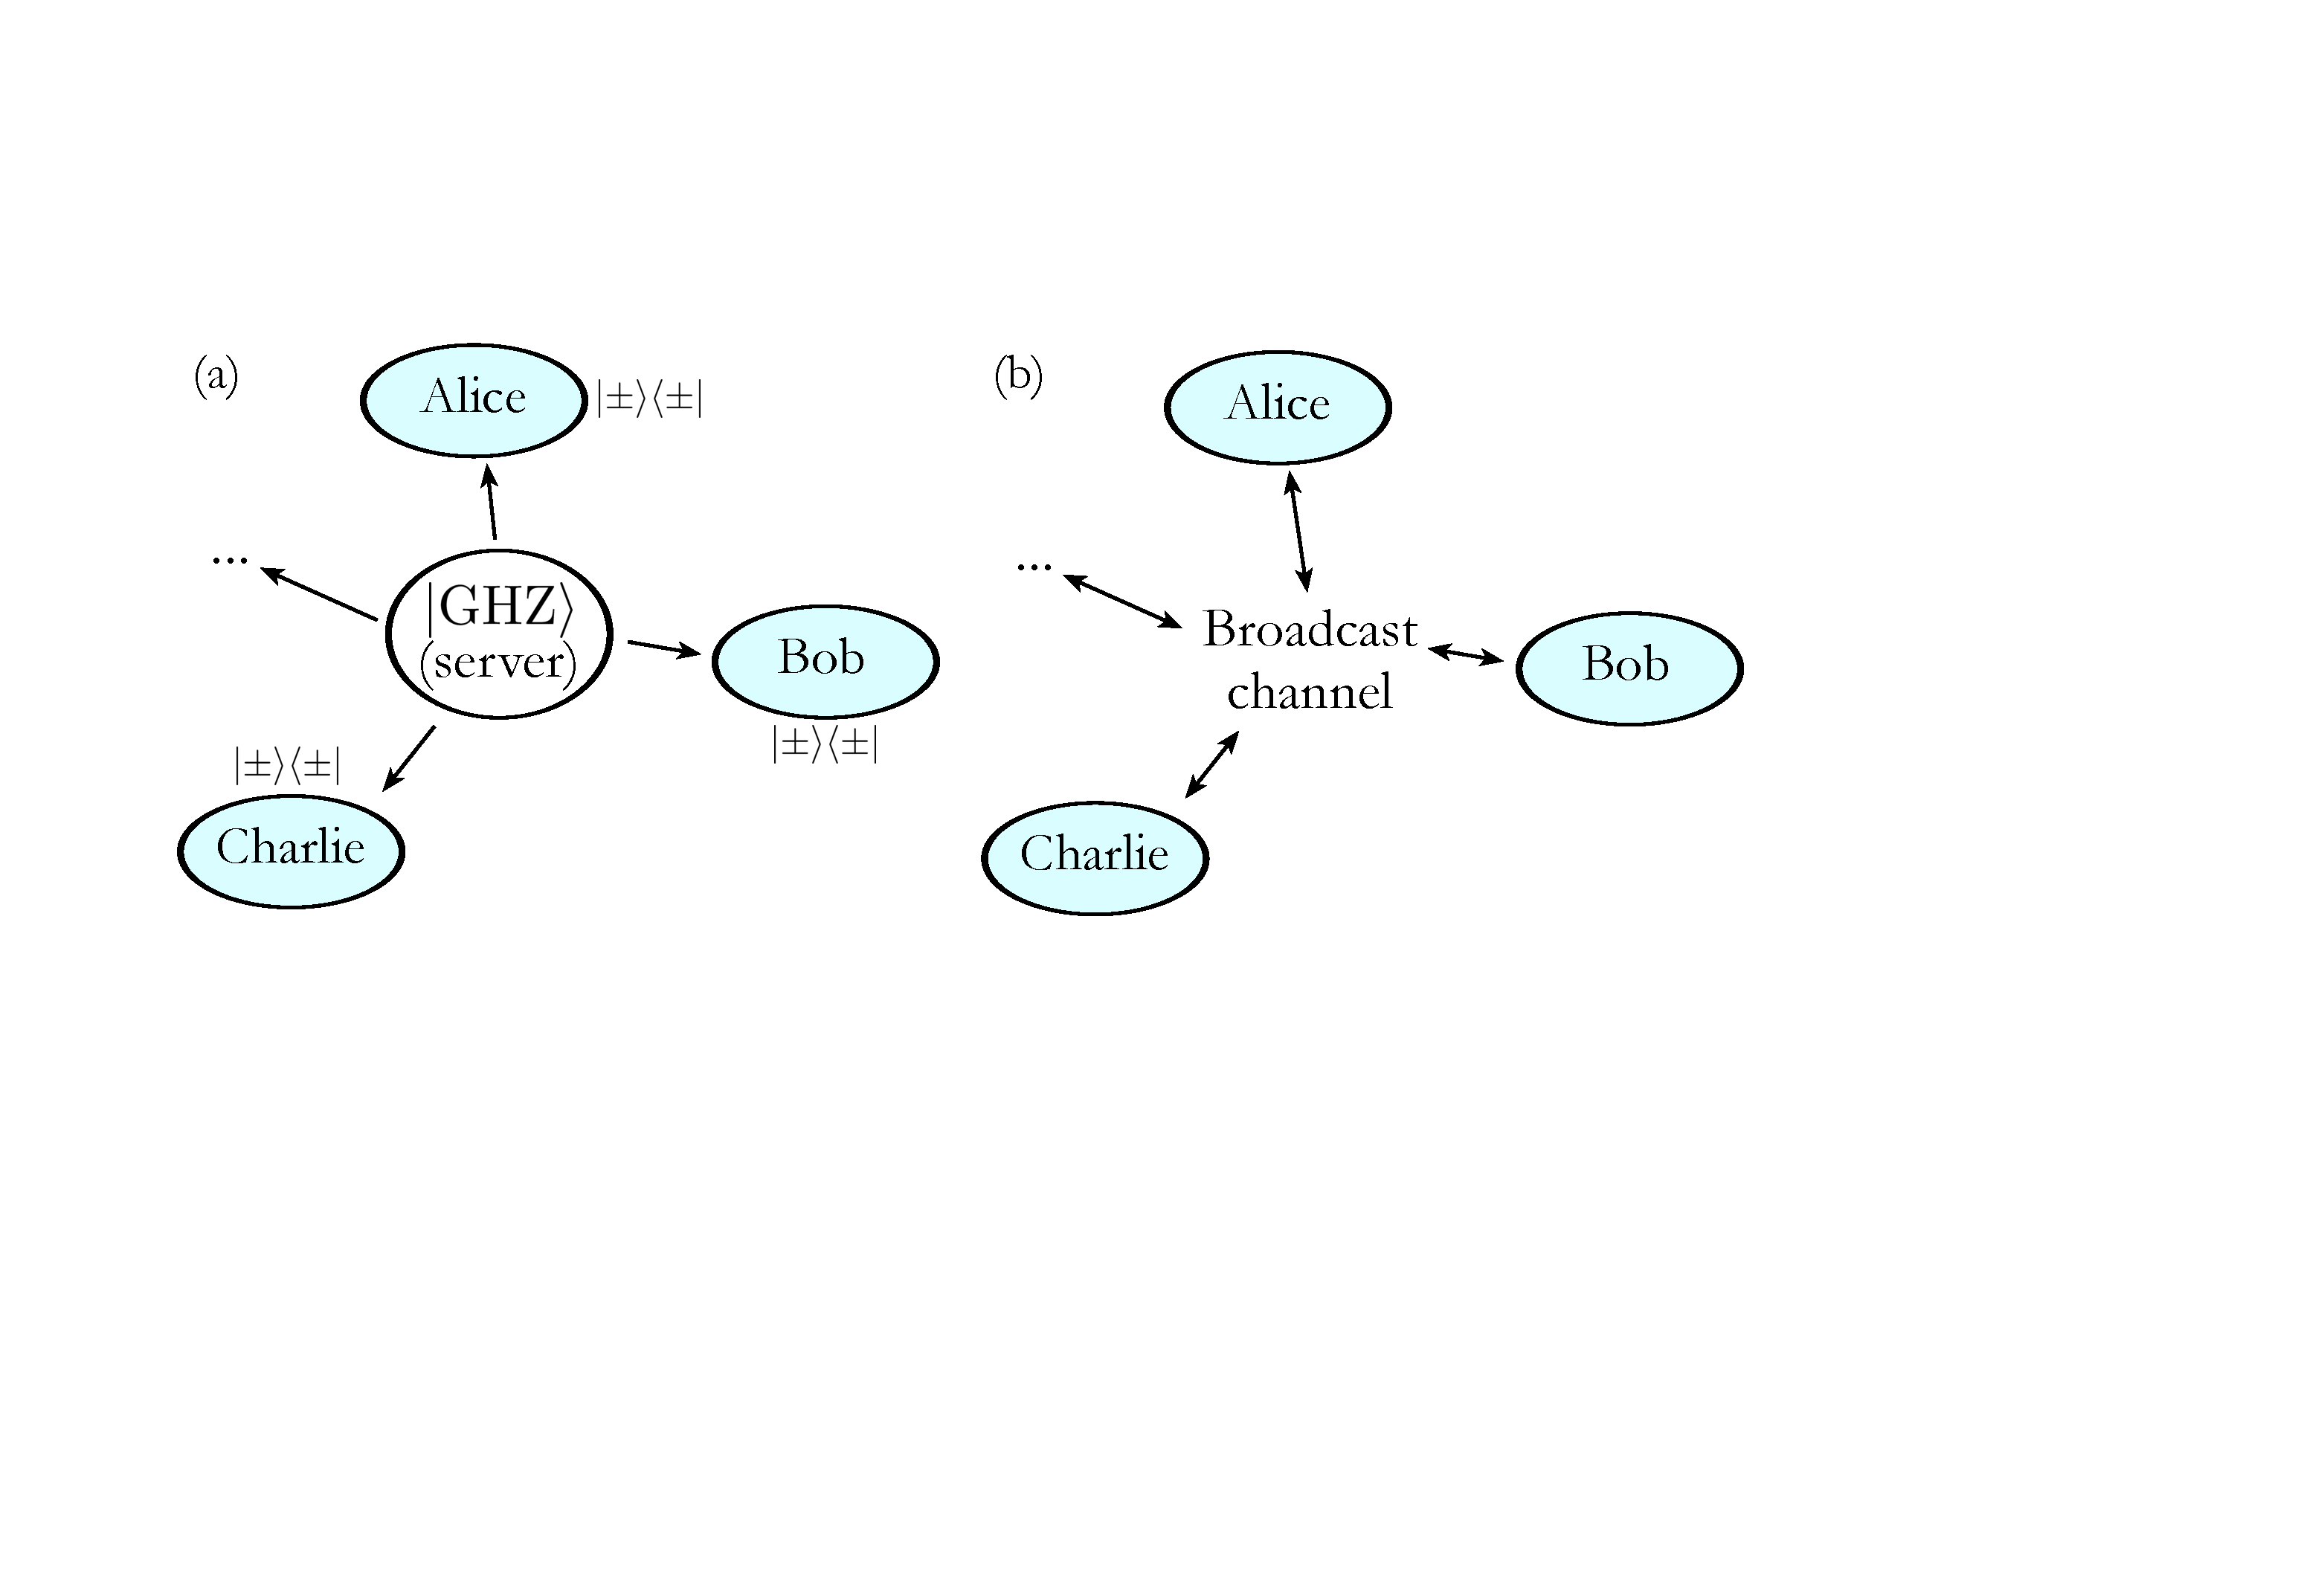
\includegraphics[width=0.47\textwidth]{QAB}
\caption{Protocol for quantum anonymous broadcasting. (a) A central trusted server prepares GHZ states and distributes them amongst a group of users, one qubit per user. All users measure in the $\pm$-basis. (b) All users classically broadcast their measurement outcomes yielding shared random parity. During broadcast, the broadcaster lies about his measurement outcome to flip the joint parity if he wishes to transmit `1', or tells the truth to transmit `0'. The joint parity encodes the message of the anonymous user, which all listeners are able to recover.} \label{fig:QAB}
\end{figure}

\begin{table}[!htb]
\fbox{\parbox{0.965\columnwidth}{\texttt{ 
function QuantumAnonymousBroadcasting(message, speaker):
\begin{enumerate}
\item $\ket\psi = \frac{1}{\sqrt{2}}(\ket{0}^{\otimes n}+\ket{1}^{\otimes n})$
\item $\ket\psi \to (\hat{Z}_\text{speaker})^\text{message}\ket\psi$
\item for(i$\in$users) \{
	\setlength{\itemindent}{.2in}
\item outcome$_i$ = measureInXBasis($\ket\psi_\text{i}$)
\setlength{\itemindent}{0in}
\item \}
\item parity = $\sum_i$ outcome$_i$\,(mod\,2)
\item return(parity)
\item $\Box$
\end{enumerate}
}}}
\caption{Protocol for quantum anonymous broadcasting. The GHZ state is distributed in advance, one qubit per user. The measurement outcomes are classically broadcast without encryption. The final parity of the classical measurements reflects the message bit without identifying the speaker.} \label{alg:QAB}
\end{table}

Note that the scheme can be slightly simplified by rather than the speaker applying the $\hat{Z}$ to his qubit, upon announcing his measurement outcome he instead simply lies about his outcome and flips it. This follows simply because a $\hat{Z}$ gate prior to a $\pm$ measurement bit flips the classical measurement outcome, \mbox{$\hat{Z}\ket\pm=\ket\mp$}.

There are no constraints on time ordering of the measurements, nor, much like BB84, are there any interferometric requirements (not including the GHZ preparation stage), making this protocol very experimentally practical and robust over long distances.

Because of the time invariance in the measurements, distribution and measurement of the GHZ states can be performed well in advance of the actual message broadcast. This allows us to treat `shared parity'\index{Shared parity} as a fundamental resource (Sec.~\ref{sec:ent_ultimate}) for the QAB cryptoprotocol.

Since the parity-sharing can be isolated from the broadcasting stage it is unimportant if the GHZ source is non-deterministic or the channels for distributing it lossy. We can instead simply repeat GHZ distribution over and over at high repetition rate, post-selecting upon measurement outcomes where all users signal that they successfully received and measured their photons.

For these reasons, this scheme lends itself readily to photonic implementation, provided a reliable GHZ preparation circuit. The scheme has since been ported to operate on distributed toric codes\index{Toric code} to facilitate error correction of the distributed GHZ states \cite{GavinMeni}.

%
% Attacks On Quantum Cryptography
%

\subsection{Attacks on quantum cryptography}

\comment{To do}

\comment{Attackes based on bad implementation rather than bad theory}